\documentclass[8pt,a4paper,compress]{beamer}

\usepackage{/home/siyer/lib/slides}

\title{Control Flow}
\date{}

\begin{document}
\begin{frame}
\vfill
\titlepage
\end{frame}

\begin{frame}
\frametitle{Outline}
\tableofcontents
\end{frame}

\section{If Statement}
\begin{frame}[fragile]
\pause

Most computations require different actions for different inputs and one way to express these differences in Python is using the \lstinline{if} statement

\pause
\smallskip

\begin{lstlisting}[language={}]
if <boolean expression>:
    <statement>
    <statement>
    ...
elif <boolean expression>:
    <statement>
    <statement>
    ...
elif <boolean expression>:
    <statement>
    <statement>
    ...
...
else: 
    <statement>
    <statement>
    ...
\end{lstlisting}
\end{frame}

\begin{frame}[fragile]
\pause

\begin{framed}
\tiny flip.py: Simulate a coin flip by writing 'Heads' or 'Tails' to standard output.
\end{framed}

\begin{lstlisting}[language=Python]
import random
import stdio

if random.randrange(0, 2) == 0:
    stdio.writeln('Heads')
else:
    stdio.writeln('Tails')
\end{lstlisting}

\pause

\begin{lstlisting}[language={}]
$ python flip.py 
Tails
$ python flip.py 
Heads
$ python flip.py 
Heads
$ python flip.py 
Tails
$ python flip.py 
Heads
\end{lstlisting}
\end{frame}

\section{While Statement}
\begin{frame}[fragile]
\pause

Many computations are inherently repetitive and the basic Python construct for handling such computations is the \lstinline{while} statement

\pause
\smallskip

\begin{lstlisting}[language={}]
while <boolean expression>:
    <statement>
    <statement>
    ...
\end{lstlisting}
\end{frame}

\begin{frame}[fragile]
\pause

\begin{framed}
\tiny tenhellos.py: Write 10 Hellos to standard output.
\end{framed}

\begin{lstlisting}[language=Python]
import stdio

stdio.writeln('1st Hello')
stdio.writeln('2nd Hello')
stdio.writeln('3rd Hello')
i = 4
while i <= 10:
    stdio.writeln(str(i) + 'th Hello')
    i = i + 1
\end{lstlisting}

\pause

\begin{minipage}{150pt}
\begin{lstlisting}[language={}]
$ python tenhellos.py 
1st Hello
2nd Hello
3rd Hello
4th Hello
5th Hello
6th Hello
7th Hello
8th Hello
9th Hello
10th Hello
\end{lstlisting}
\end{minipage}\hfill
\begin{minipage}{100pt}
Variable trace
\begin{lstlisting}[language={}]
i     output
----------------

4     4th hello
5     5th hello
6     6th hello
7     7th hello
8     8th hello
9     9th hello
10    10th hello
11
\end{lstlisting}
\end{minipage}
\end{frame}

\begin{frame}[fragile]
\pause

\begin{framed}
\tiny powersoftwo.py: Accept positive integer $n$ as a command-line argument. Write to standard output a table showing the first $n$ powers of two.
\end{framed}

\begin{lstlisting}[language=Python]
import stdio
import sys

n = int(sys.argv[1])
power = 1
i = 0
while i <= n:
    stdio.writeln(str(i) + ' ' + str(power))    
    power = 2 * power
    i = i + 1
\end{lstlisting}

\pause

\begin{minipage}{150pt}
\begin{lstlisting}[language={}]
$ python powersoftwo.py 8
0 1
1 2
2 4
3 8
4 16
5 32
6 64
7 128
8 256
\end{lstlisting}
\end{minipage}\hfill
\begin{minipage}{100pt}
Variable trace (\lstinline{n = 8})
\begin{lstlisting}[language={}]
power    i    output
--------------------
1        0    0 1
2        1    1 2
4        2    2 4
8        3    3 8
16       4    4 16
32       5    5 32
64       6    6 64
128      7    7 128
256      8    8 256
512      9
\end{lstlisting}
\end{minipage}
\end{frame}

\begin{frame}[fragile]
\pause

Modifying a variable is something that we do so often that Python provides shorthand notations for the purpose

\pause
\bigskip

The most common practice is to abbreviate an assignment statement of the form 

\begin{lstlisting}[language=Python]
i = i + 1
\end{lstlisting}

with the shorthand notation

\begin{lstlisting}[language=Python]
i += 1
\end{lstlisting}

\pause
\bigskip

The same notation works for other binary operators, including \lstinline{-}, \lstinline{*}, and \lstinline{/}

\pause
\bigskip

The scope of a variable is part of the program where it is defined, ie, statements that follow the definition in the same block (marked by indentation level)
\end{frame}

\section{For Statement}
\begin{frame}[fragile]
\pause

The \lstinline{for} statement provides a more compact notation for carrying out repeated computations

\pause
\smallskip

\begin{lstlisting}[language={}]
for <variable> in <iterable object>:
    <statement>
    <statement>
    ...
\end{lstlisting}

\pause
\bigskip

The most commonly used iterable objects are the lists containing arithmetic progressions of integers, returned by the built-in function \lstinline{range()}

\pause
\bigskip

The call \lstinline{range(start, stop[, step])} returns a list starting at \lstinline{start}, ending just before \lstinline{stop}, and in increments (or decrements) given by the optional \lstinline{step} argument, which defaults to 1

\pause
\bigskip

The call \lstinline{range(stop)} is shorthand for \lstinline{range(0, stop)}

\pause
\bigskip

For example
\begin{lstlisting}[language={}]
range(8, 0, -2) = [8, 6, 4, 2]

range(3, 9)     = [3, 4, 5, 6, 7, 8]

range(5)        = [0, 1, 2, 3, 4]
\end{lstlisting}
\end{frame}

\begin{frame}[fragile]
\pause

The \lstinline{tenhellos.py} program can be written using a \lstinline{for} statement as follows

\begin{lstlisting}[language=Python]
import stdio

stdio.writeln('1st Hello')
stdio.writeln('2nd Hello')
stdio.writeln('3rd Hello')
for i in range(4, 11):
    stdio.writeln(str(i) + 'th Hello')
\end{lstlisting}

\pause
\bigskip

Strings are iterable objects, so its characters can be enumerated using a for loop 

\pause
\bigskip

For example, the following code
\begin{lstlisting}[language=Python]
import stdio

for c in 'AGCT':
    stdio.writeln(c)
\end{lstlisting}

produces the output

\begin{lstlisting}[language={}]
A
G
C
T
\end{lstlisting}
\end{frame}

\section{Nesting}
\begin{frame}[fragile]
\pause

The \lstinline{if}, \lstinline{while}, and \lstinline{for} statements, collectively called control-flow statements, have the same status as assignment statements or any other statements in Python

\pause
\bigskip

As a result, we can use a control-flow statement whenever a statement is called for

\pause
\bigskip

In particular, we can nest one or more of the control-flow statements in the body of another
\end{frame}

\begin{frame}[fragile]
\pause

\begin{framed}
\tiny divisorpattern.py: Accept integer command-line argument $n$. Write to standard output an $n$-by-$n$ table with an asterisk in row $i$ and column $j$ if either $i$ divides $j$ or $j$ divides $i$.
\end{framed}

\begin{lstlisting}[language=Python]
import stdio
import sys

n = int(sys.argv[1])
for i in range(1, n + 1):
    for j in range(1, n + 1):
        if (i % j == 0) or (j % i == 0):
            stdio.write('* ')
        else:
            stdio.write('  ')
    stdio.writeln(i)
\end{lstlisting}

\pause

\begin{minipage}{150pt}
\begin{lstlisting}[language={}]
$ python divisorpattern.py 3
* * * 1
* *   2
*   * 3
\end{lstlisting}
\begin{lstlisting}[language={}]
$ python divisorpattern.py 10
* * * * * * * * * * 1
* *   *   *   *   * 2
*   *     *     *   3
* *   *       *     4
*       *         * 5
* * *     *         6
*           *       7
* *   *       *     8
*   *           *   9
* *     *         * 10
\end{lstlisting}
\end{minipage}\hfill
\begin{minipage}{100pt}
Variable trace (\lstinline{n = 3})
\begin{lstlisting}[language={}]
i    j    output
----------------
1    1    '* '
1    2    '* '
1    3    '* 1\n'
2    1    '* '
2    2    '* '
2    3    ' 2\n'
3    1    '* '
3    2    '  '  
3    3    '* 3\n'
\end{lstlisting}
\end{minipage}
\end{frame}

\section{Applications}
\begin{frame}[fragile]
\pause

\begin{framed}
\tiny harmonic.py: Accept integer $n$ as a command-line argument. Write to standard output the $n$th harmonic number $H_n$, computed as $H_n=1+1/2+1/3+\cdots+1/n$. Note that $H_n \approx \ln(n) + 0.57721$ for large $n$.
\end{framed}

\begin{lstlisting}[language=Python]
import stdio
import sys

n = int(sys.argv[1])
total = 0.0
for i in range(1, n + 1):
    total += 1.0 / i
stdio.writeln(total)
\end{lstlisting}

\pause

\begin{lstlisting}[language={}]
$ python harmonic.py 2
1.5
$ python harmonic.py 10
2.92896825397
$ python harmonic.py 10000
9.78760603604
\end{lstlisting}
\end{frame}

\begin{frame}[fragile]
\pause

\begin{framed}
\tiny sqrt.py: Accept a float $c$ as a command-line argument. Write to standard output the square root of $c$ to 15 decimal places of accuracy, calculated using Newton's method.
\end{framed}

\begin{minipage}{150pt}
\begin{lstlisting}[language=Python]
import stdio
import sys

EPSILON = 1e-15
c = float(sys.argv[1])
t = c
while abs(1 - c / t ** 2) > EPSILON:
    t = (c / t + t) / 2.0
stdio.writeln(t)
\end{lstlisting}
\end{minipage}%
\begin{minipage}{150pt}
\hfill \visible<2->{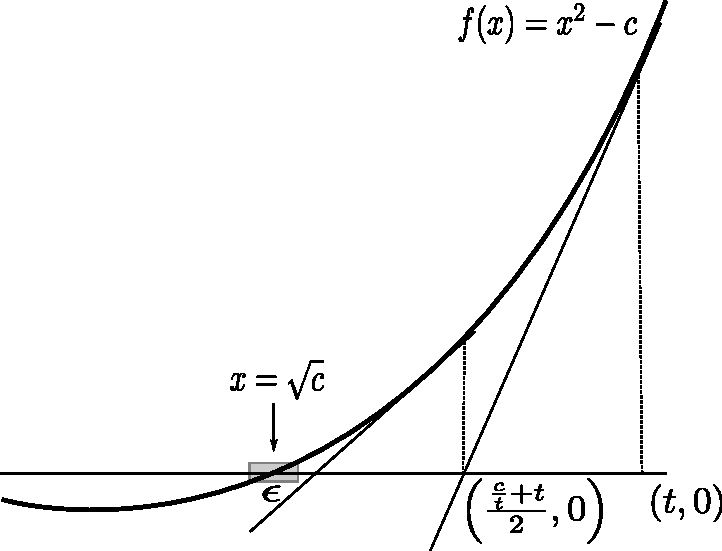
\includegraphics[scale=0.4]{figures/sqrt.pdf}}
\end{minipage}

\pause

\begin{lstlisting}[language={}]
$ python sqrt.py 2.0
1.41421356237
$ python sqrt.py 2544545
1595.16300108
\end{lstlisting}
\end{frame}

\begin{frame}[fragile]
\pause

\begin{framed}
\tiny binary.py: Accept integer $n$ as a command-line argument. Write the binary representation of $n$ to standard output.
\end{framed}

\begin{minipage}{150pt}
\begin{lstlisting}[language=Python]
import sys
import stdio

n = int(sys.argv[1])
v = 1
while v <= n // 2:
    v *= 2
while v > 0:
    if n < v:
        stdio.write(0)
    else:
        stdio.write(1)
        n -= v
    v //= 2
stdio.writeln()
\end{lstlisting}

\end{minipage}%
\begin{minipage}{150pt}
\hfill \visible<2->{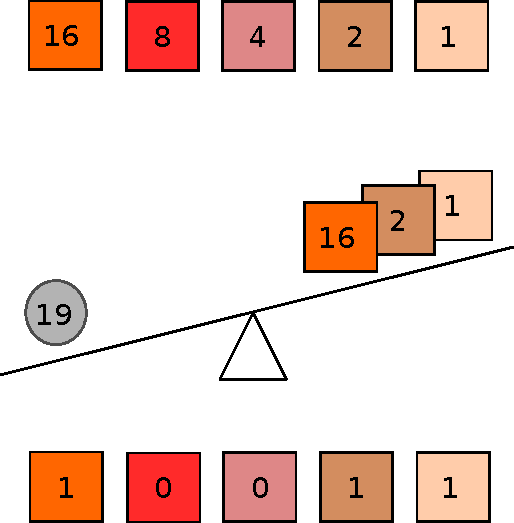
\includegraphics[scale=0.4]{figures/binary.pdf}}
\end{minipage}

\pause

\begin{lstlisting}[language={}]
$ python binary.py 19
10011
$ python binary.py 255
11111111
$ python binary.py 512
1000000000
$ python binary.py 1000000000
111011100110101100101000000000
\end{lstlisting}
\end{frame}

\begin{frame}[fragile]
\pause

\begin{framed}
\tiny gambler.py: Accept integer command-line arguments $stake$, $goal$, and $trials$. Run $trials$ experiments that start with $stake$ dollars and terminate on 0 dollars or $goal$. Write to standard output the percentage of wins and the average number of bets per experiment, which can be calculated as $100 \times stake / goal$ and $stake \times (goal - stake)$, respectively.
\end{framed}

\begin{minipage}{200pt}
\begin{lstlisting}[language=Python]
import random
import stdio
import sys

stake = int(sys.argv[1])
goal = int(sys.argv[2])
trials = int(sys.argv[3])
bets = 0
wins = 0
for t in range(trials):
    cash = stake
    while cash > 0 and cash < goal:
        bets += 1
        if random.randrange(0, 2) == 0:
            cash += 1
        else:
            cash -= 1
    if cash == goal:
        wins += 1
stdio.writeln(str(100 * wins // trials) + '% wins')
stdio.writeln('Avg # bets: ' + str(bets // trials))
\end{lstlisting}
\end{minipage}%
\begin{minipage}{100pt}
\hfill \visible<2->{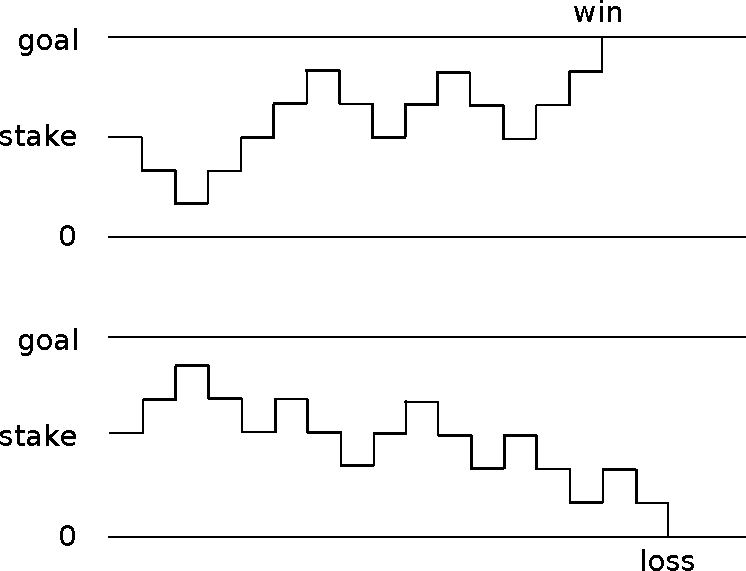
\includegraphics[scale=0.3]{figures/gambler.pdf}}
\end{minipage}

\pause

\begin{lstlisting}[language={}]
$ python gambler.py 50 250 100
24% wins
Avg # bets: 12548
$ python gambler.py 500 2500 100
27% wins
Avg # bets: 1124855
\end{lstlisting}
\end{frame}

\begin{frame}[fragile]
\pause

\begin{framed}
\tiny factors.py: Accept integer $n$ as a command-line argument. Write to standard output the prime factors of $n$.
\end{framed}

\begin{lstlisting}[language=Python]
import stdio
import sys

n = int(sys.argv[1])
factor = 2
while factor * factor <= n:
    while n % factor == 0:
        n //= factor
        stdio.write(str(factor) + ' ')
    factor += 1
if n > 1:
    stdio.write(n)
stdio.writeln()
\end{lstlisting}

\pause

\begin{lstlisting}[language={}]
$ python factors.py 3757208
2 2 2 7 13 13 397
$ python factors.py 287994837222311
17 1739347 9739789
\end{lstlisting}
\end{frame}

\section{Other Conditional and Loop Constructs}
\begin{frame}[fragile]
\pause

The conditional expression supports an alternate form of an \lstinline$if-else$ statement
 
\begin{lstlisting}[language={}]
<expression> if <boolean expression> else <expression>
\end{lstlisting}

For example, the following code assigns \lstinline{'Heads'} or \lstinline{'Tails'} to the variable \lstinline{flip}, each with probability $1/2$

\begin{lstlisting}[language=Java]
flip = 'Heads' if random.random() < 0.5 else 'Tails'
\end{lstlisting}

\pause
\bigskip

The \lstinline{break} statement immediately exits a loop without letting it to run to completion

\pause
\bigskip

For example, the following code tests and prints if a number $N$ is prime or not
\begin{lstlisting}[language=Python]
i = 2
while i <= N / i:
    if N % i == 0:
        break
    i += 1
stdio.writeln(str(N) + (' is ' if i > N / i else ' is not ') + 'prime')
\end{lstlisting}

\pause
\bigskip

The \lstinline{continue} statement skips to next iteration of a loop

\pause
\bigskip

For example, the following code iterates over the characters in the English alphabet and prints only the consonants
\begin{lstlisting}[language=Python]
for c in 'abcdefghijklmnopqrstuvwxyz':
    if c == 'a' or c == 'e' or c == 'i' or c == 'o' or c == 'u':
        continue
    stdio.writeln(c)
\end{lstlisting}
\end{frame}
\end{document}
